\subsection{Admissibility}\label{sec:admissible-proof}

Our heuristics are not \emph{consistent}, but we show that a weaker variant
holds for states \emph{at the start of a seed}.

\begin{definition}[Start of seed]
A state $\st ij$ is \emph{at the start of some seed} when~$i$ is a multiple
of the seed length $k$, or when~$i=n$.
\end{definition}

\begin{lem}[Weak triangle inequality]\label{lem:weaktriangle} For states $u$,
  $v$, and $w$ with $v$ and $w$ at the starts of some seeds, all $\gamma \in
  \{\seedcost, \gapcost, \gscost\}$ satisfy
  \begin{equation*}
  {\gamma(u, v) +
  \gamma(v, w) \geq \gamma(u, v)}.
  \end{equation*}
\end{lem}
\begin{proof}
  Both $v$ and $w$ are at the start of some seeds, so for $\gamma=\seedcost$ we
  have the equality $\seedcost(u, w) = \seedcost(u, v) + \seedcost(v, w)$.

  For $\gamma = \gapcost$,
  \begin{align*}
    &\gapcost(\st ij, \st {i'}{j'}) + \gapcost(\st{i'}{j'}, \st{i''}{j''})\\
    =\ &
    |(i'-i) - (j'-j)| + |(i''-i') - (j''-j')|\\
    \geq\ &
    |(i''-i)-(j''-j)| = \gapcost(\st ij, \st{i''}{j''}).
  \end{align*}

  And lastly, for $\gamma=\gscost$,
  \begin{align*}
  &\gscost(u, v) + \gscost(v, w)\\
  = &\max(\gapcost(u,v), \seedcost(u, v)) + \max(\gapcost(v, w), \seedcost(v, w))\\
  \geq &\max(\gapcost(u, v)+ \gapcost(v, w), \seedcost(u, v) + \seedcost(v, w))\\
  \geq &\max(\gapcost(u, w), \seedcost(u, w))
  = \gscost(u, w). \qedhere
  \end{align*}
\end{proof}

\begin{lem}[Weak consistency]\label{lem:weakconsistency}
  Let $h\in \{\hshM, \hcshM, \hgchM\}$ be a heuristic with partial order
  $\preceq_p$, and let $u \preceq_p v$ be states with $v$ at the start of a seed.
  When there is a shortest path $\Path$ from $u$ to $v$ such that $\matches$
  contains all matches of cost less than $r$ on $\Path$, it holds that
  $h(u) \leq \d(u, v) + h(v)$.
\end{lem}
\begin{proof}
  The path $\Path$ covers each seed in $\substr \seeds uv$ that must to be fully
  aligned between $u$ and $v$. Since the seeds do not overlap, their shortest
  alignments $\Path_s$ in $\Path$ do not have overlapping edges. Let $u\preceq
  m_1 \preceq_p \dots \preceq_p m_{l} \preceq_p v$ be the chain of matches $m_i
  \in \matches$ corresponding to those $\Path_s$ of cost less than
  $r$~(\cref{fig:recursive-h}). Since the matches and the paths between them are
  disjoint, $\pathcost(\Path)$ is at least the cost of the matches
  $\matchcost(m_{i+1}) = \d(\start(m_{i+1}), \matchend(m_{i+1}))$ plus the cost
  to chain these matches $\gamma(\matchend(m_i), \matchstart(m_{i+1})) \leq
  \d(\matchend(m_i), \start(m_{i+1}))$. Putting this together:
  \begin{align*}
    &\gamma(u, m_1) + \matchcost(m_1) + \dots + \matchcost(m_l) + \gamma(m_l, v)\\
    \leq\ &\d(u, \start(m_1)) + \d(\start(m_1), \matchend(m_1)) + \dots +
          \d(\matchend(m_l), v)\\
    \leq\ & \d(u, v).
  \end{align*}
  Now let $v\preceq_p m_{l+1} \preceq_p \dots \preceq_p m_{l'} \preceq_p v_t$ be a chain of
  matches minimizing $h(v)$ (\cref{dfn:h}) with $w:= \start(m_{l+1})$. This
  chain also minimizes $h(w)$ and thus $h(v) = \gamma(v, w) + h(w)$. We can now
  bound the cost of the joined chain from $u$ to $v$ and from $w$ to the end and
  get our result via $\gamma(m_l, w) \leq \gamma(m_l, v) + \gamma(v, w)$ (\cref{lem:weaktriangle})
  \begin{align*}
    h(u)
    &\leq\gamma(u, m_1) + \dots+\gamma(m_l, m_{l+1}) +\matchcost(m_{l+1}) + \dots + \gamma(m_{l'}, v_t)\\
    &= \gamma(u, m_1) + \dots + \gamma(m_l, w) \hspace{1.5em}+ h(w)\\
    &\leq \gamma(u, m_1) + \dots + \gamma(m_l, v) + \gamma(v, w)+(h(v)-\gamma(v, w))\\
    &\leq \d(u, v) + h(v). && \tag*{\qed}
  \end{align*}
  \let\qed\relax
\end{proof}

\begin{figure}[H]
    \centering
    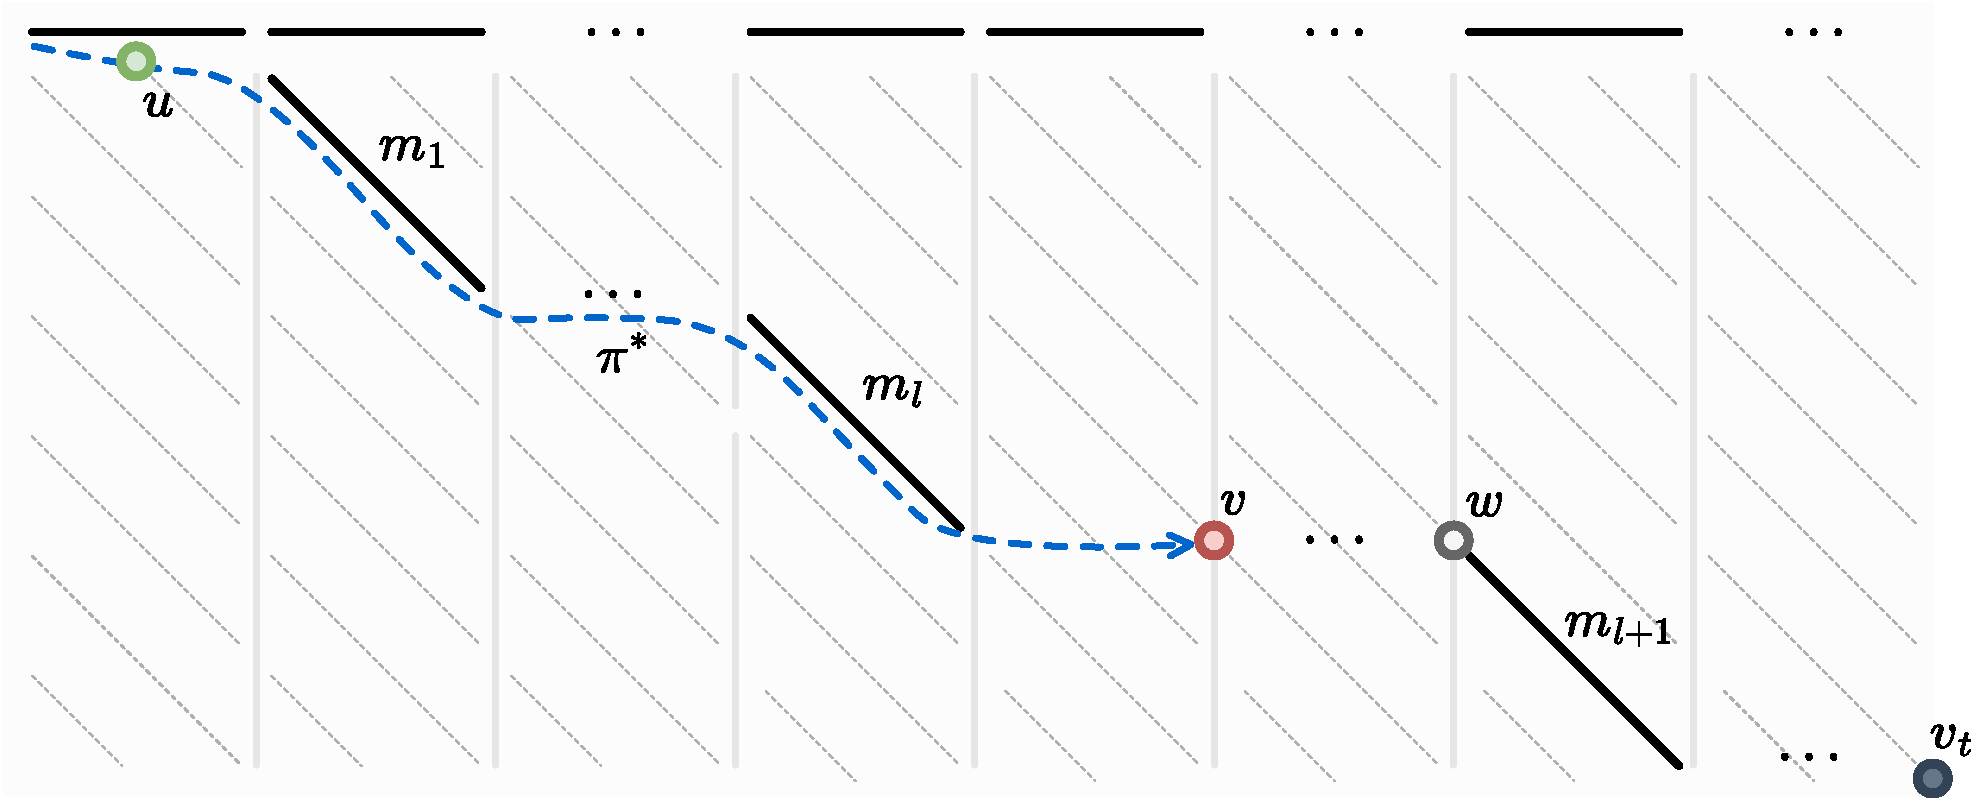
\includegraphics[width=0.8\linewidth]{imgs/proofs/recursive-h.pdf}%
    \caption[Variables of the proof of \cref{lem:weakconsistency}.]{\textbf{Variables of the proof of \cref{lem:weakconsistency}.}}
    \label{fig:recursive-h}
\end{figure}

\thmadmissible*
\begin{proof}
  We will prove $\hshM(u) {\overset{(1)}{\leq}} \hcshM(u) {\overset{(2)}{\leq}}
  \hgchM(u) {\overset{(3)}{\leq}} \h(u)$, which implies the admissibility of
  all three heuristics.

  (1) Note that $u\preceq v$ implies $u\preceq_i v$ and hence any
  $\preceq$-chain is also a $\preceq_i$-chain. A minimum over the superset of
  $\preceq_i$-chains is at most the minimum of the subset of $\preceq$-chains,
  and hence $\hshM = h^{\matches}_{\preceq_i, \seedcost} \leq
  h^{\matches}_{\preceq, \seedcost} = \hcshM$.
  
  (2) The only difference between $\hcshM$ and $\hgchM$ is that the
  former uses $\seedcost$ and the latter uses the gap-seed cost $\gscost :=
  \max(\gapcost, \seedcost)$. Since $\seedcost \leq \gscost$ we have $\hcshM =
  h^{\matches}_{\preceq, \seedcost} \leq h^{\matches}_{\preceq, \gscost} =
  \hgchM$.

  (3)
  When $\matches$ is the set of all matches with costs strictly less than $r$,
  admissibility follows directly from \cref{lem:weakconsistency} with $v = v_t$
  via
  \begin{equation*}
  \hgchM(u) \leq \d(u, v_t) + \hgchM(v_t) = \d(u, v_t) = \h(u).\qedhere
  \end{equation*}
\end{proof}
